\chapter{Deuxième principe de la thermodynamique}

L'un des objectifs de la thermodynamique est de prédire le sens d'évolution d'un système, si une contrainte est levée. Le premier principe, n'impose pas le signe du travail et de la chaleur, alors que le signe est normalement imposé.\\

Un moteur monotherme est une machine thermique, en contact avec une unique source de chaleur. On aura un travail négatif (donc moteur), ce qui impliquera que la chaleur est égale à l'opposé du travail, du fait que nous ayons un cycle, impliquant une énergie interne nulle. Or, cette condition théorique impose que le transfert de chaleur soit positif, mais l'expérience nous montre l'inverse, puisque la température de notre moteur est supérieure à la température ambiante, il y a donc là contradiction.\\

Face à cette contradiction, il a fallut développer un principe capable de donner le sens d'évolution des transformations.

\section{Transformations réversibles}

Une transformation réversible se fait entre deux états initiaux et finaux tel qu'entre ces états, il existe des états d'équilibre thermodynamique. A contrario, l'irréversibilité correspond à une transformation qui ne peut être faite en sens inverse. C'est le cas de l'application des forces de frottements, qui dissipent l'énergie par de l'énergie thermique, induisant une libération de chaleur.\\

L'énoncé de Clausius dit :

\begin {center}
\textit{"Une quantité de chaleur ne peut jamais être transférée spontannément d'une source froide vers une source chaude."}
\end{center}

Kelvin lui énoncera le fait que :
\begin{center}
\textit{"Il est impossible de prélever une quantité de chaleur d'une source d'énergie, et de la transformer intégralement en travail."}
\end{center}

C'est l'incapacité de transformer la chaleur en travail, qui a forcé les scientifiques à introduire une nouvelle fonction d'état. La fonction d'état du second principe est \textbf{l'entropie}.

\begin{definition}[Entropie]
L'entropie est une variable d'état extensive, notée $S$, et qui permet de mesurer le désordre dans un système. Son unité est le $J.K^{-1}$. La principale relation à laquelle on peut la corréler, en particulier avec la température et la chaleur est

\begin{equation}
\delta Q=TdS
\end{equation}

\end{definition}



\section{Echange et création d'entropie}

On considère un système fermé en contact avec une source de chaleur, de température $T_e$. On peut alors utiliser le deuxième principe de la thermodynamique.
\begin{theorem}[Deuxième principe de la thermodynamique]
La variation d'élémentaire d'entropie est égale à la somme de l'entropie échangée ainsi que l'entropie créée. On a ainsi
\begin{equation}
dS=\delta S_e + \delta S_c
\end{equation}
\end{theorem}
On introduit ici deux termes, le premier $\delta S_e$ correspond à l'entropie échangée, et $\delta S_c$, l'entropie créée ne pouvant prendre que deux valeurs : $\delta S_c = 0$ ou $\delta S_c > 0$. Dans ces deux cas, on aura repectivement, soit une transformation réversible, soit une tansformation irréversible. En aucun cas, \textbf{l'entropie créée} ne peut être négative.\\

\begin{proposition}[Création d'entropie]
Au cours d'une transformation, de l'entropie peut être créée, représentée par le $\delta S_c$, mais l'entropie ne peut jamais disparaître. Pour une transformation réversible, on aura une entropie créée nulle et sinon, elle est positive.
\end{proposition}

Ainsi, entre deux états $A$ et $B$, on a
\begin{equation}
\Delta S_A^B=S_c+S_e=S_c+\int \frac{\delta Q_e}{T_e}
\end{equation}

Pour une transformation réversible, on a $S_c=0$
\begin{equation}
\Delta S_A^B=S_e=\int \limits_A^B \frac{\delta Q_{rev.}}{T}
\end{equation}

Pour une transfroamtion irréversible, on a $S_c>0$
\begin{equation}
S_e=\int \limits_A^B \frac{\delta Q_{irr.}}{T}
\end{equation}

Dans le cadre d'un système isolé, on a $Q_e=0$, donc
\begin{equation}
\Delta S = S_c >0
\end{equation}
On en déduit que l'entropie dans un système fermé, ne peut qu'augmenter.\\

\begin{proposition}[Evolution du désordre dans un système isolé]
Dnas un système isolé, toute transformation irréversible est vouée à créer de l'entropie et donc du désordre. Ainsi, un tel système ne peut pas voire son entropie décroître
\end{proposition}

On notera que si on a $\Delta S=0$, cela implique qu'on a une transformation réversible adiabatique, puisque les entropies créées et échangées sont nulles. C'est un cas particulier de \textbf{transformation isentropique}, c'est-à-dire à entropie constante.\\

Si on a un soldie en contact thermique, on note que, à l'état initial, on a deux températures différentes entre nos objets, $T_A$ pour notre solide, et $T_E$ pour notre source de chaleur. A l'équilibre, on aura alors pour chaleur reçue
$$Q=\int \delta Q = \int \limits_A^E CdT$$
$$\Leftrightarrow Q = C(T_E-T_A)$$

L'entropie échangée, elle, vaut
$$S_e=\int \frac{\delta Q_e}{T_E}=\frac{1}{T_E}\int \delta Q_e=\frac{C(T_e-T_a)}{T_e}$$

Finalement, comme $S$ est une fonction d'état, on a
$$\Delta S = S_e + S_c = S_f-S_i$$

Si maintenant on imagine une transformation réversible, on peut représenter la situation tel le schéma suivant :

\begin{figure}[H]
\centering
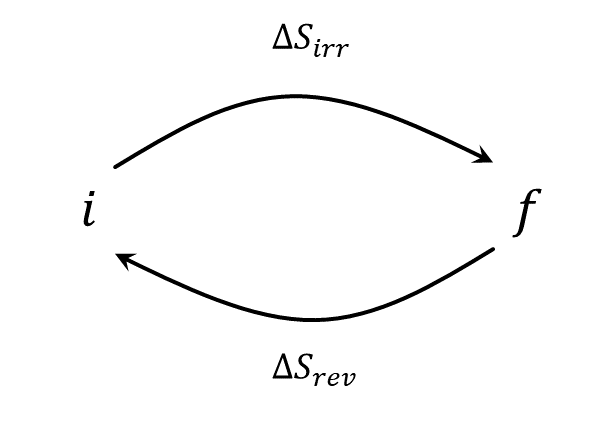
\includegraphics[scale=0.6]{Diapositiv5.png}
\caption{Transformations réversibles et irréversibles}
\end{figure}

Dans cette situation, on a 
$$\Delta S_{irr} = \Delta S_{rev}$$
Or, on a
$$\Delta S_{irr}=\int \limits_A^B \frac{\delta Q}{T}=\int \limits_A^B \frac{CdT}{T}=C \ln \left ( \frac{T_E}{T_A} \right )$$
Finalement, on en déduit que
$$\Delta S_{irr}=C \frac{T_E-T_A}{T_E} + S_c = C \ln \frac{T_E}{T_A}$$
\begin{proposition}[Entropie créée au cours d'une transformation irréversible]
Pour une transformation irréversible, l'entropie crée s'écrit
\begin{equation}
S_c = C \ln \frac{T_E}{T_A} - C \frac{T_E-T_A}{T_E}
\end{equation}
\end{proposition}

\section{Identité thermodynamique}

A partir du premier principe, on a 
$$dU=\delta Q+ \delta W$$
D'autre par, on a 
$$\delta Q = TdS$$
On en déduit la différentielle totale de l'énergie interne à partir de l'entropie.
\begin{proposition}[Différentielle totale entropique de l'énergie interne]
\begin{equation}
dU=TdS -PdV
\end{equation}
\end{proposition}
\begin{proposition}[Différentielle par dérivées partielles entropique de l'énergie interne]
\begin{equation}
dU=\left ( \frac{\partial U}{\partial S}\right )_V dS + \left ( \frac{\partial U}{\partial V} \right ) _ S dV
\end{equation}
\end{proposition}

On en déduit donc que la température peut aussi s'écrire
\begin{equation}
T=\left ( \frac{\partial U}{\partial S}\right )_V
\end{equation}

Dans la cas d'un gaz parfait, on a 
$$dU = C_v dT \textrm{ et } P=\frac{nRT}{V} \Rightarrow dS=\frac{dU}{T}+\frac{P}{T}dV$$
On peut ainsi en déduire la notation en différentielle totale
\begin{proposition}[Différentielle entropique des gaz parfaits]
\begin{equation}
dS=C_v\frac {dT}{T}+nR\frac{dV}{V}
\end{equation}
\end{proposition}
Ce qui implique, que pour un gaz parfait, on a
\begin{eqnarray}
\Delta_{GP} S = nC_v \ln \frac{T_1}{T_0} + nR \ln \frac{V_1}{V_0}\\
\Delta_{GP} S = nC_p \ln \frac{T_1}{T_0} - nR \ln \frac{P_1}{P_0}
\end{eqnarray}

Les capacités calorifiques dans ce cadre doivent être exprimées
$$dU = \delta W + \delta Q \Leftrightarrow dU=\delta Q -PdV$$
On en déduit


$$\delta Q = dU + PdV$$
 $$= \left ( \frac{\partial U}{\partial T}\right ) _V dT + \left ( \frac{\partial U}{\partial V}\right )_T dV + PdV$$
 $$= \left ( \frac{\partial U}{\partial T}\right ) _V dT + \left ( \left ( \frac{\partial U}{\partial V}\right)_T+P \right ) dV$$
 
 On a ainsi
 $$C_v=\left ( \frac{\partial U}{\partial T}\right ) _V ~~~~ l=P+\left ( \frac{\partial U}{\partial V}\right )_T ~~~~ h=\left ( \frac{\partial H}{\partial P}\right ) _T -V$$


 On peut ainsi en déduire
 \begin{equation}
 \left \{ \begin{array}{c c} \delta Q_v &= C_vdT + ldV\\ \delta Q_p &= C_pdT + hdP \end{array} \right.
 \end{equation}
 
 A partir de ces équations, on a
 $$dU = \delta Q - PdV = C_vdT(l-P)dV$$
 $$dS=\frac{\delta Q}{T} = \frac{C_vdT}{T}+\frac{l}{T}dV$$
$$\Rightarrow \frac{C_v}{T} = \left ( \frac{\delta S}{dT}\right ) _V$$
Finalement, on a 
\begin{equation}
C_v=T\left ( \frac{\partial S}{\partial T}\right ) _V \textrm{    et    }C_p=T\left ( \frac{\partial S}{\partial T} \right )_P
\end{equation}

\begin{definition}[Coefficient thermodynamiques]

 On peut résumer l'ensemble des coefficient thermodynamiques vu jusqu'ici en llien avec l'entropie
$$C_v = \left ( \frac{\partial S}{\partial T}\right ) _ V = \left ( \frac{\partial U}{\partial T}\right ) _ V$$
$$l = T \left ( \frac{\partial S}{\partial V} \right ) _T = P + \left ( \frac{\partial U }{\partial V}\right ) _T$$
$$C_p = T\left ( \frac{\partial S}{\partial T}\right ) _P = \left ( \frac{\partial H }{\partial T}\right ) _P$$
$$h = T\left ( \frac{\partial S}{\partial P}\right )_T = \left ( \frac{\partial H}{\partial P}\right )_T-V$$
\end{definition}

\section{Critères d'évolution spontannée}

\subsection{Transformation spontannée}


On note que pour un système isolé $\delta Q=0$.\\

Par définition, pour un système isolé, l'entropie de notre système ne peut que croître. Souvent, on associe l'irréversibilité à la spontanéité d'une transformation. Ainsi, on rappele que
$$dS= \delta S_e +\delta S_c$$
$$dS=\frac{\delta Q}{T}+\delta S_c$$
Pour une transformation réversible, on a 
$$\delta S_c =0 \Rightarrow dS=\frac{\delta Q_{rev}}{T}$$
Pour une transformation irréversible, on a 
$$\delta S_c > 0 \textrm{ et } \delta S_e =\frac{\delta Q_{irr}}{T}$$
Finalement, on a 
$$dS= \frac{\delta Q_{irr}}{T} + \delta S_c \Leftrightarrow dS - \frac{\delta Q_{irr}}{T}=\delta S_c >0$$
Donc 
$$dS>\frac{\delta Q_{irr}}{T} \Leftrightarrow dS \geq \frac{\delta Q}{T}$$

On en déduit que $TdS \geq \delta Q$ , pour $P=cste$, on a $\delta Q_p=dH$ donc $TdS \geq dH$. \\

On peut donc écrire que $dH-TdS \leq 0$ soit $d(TS)=TdS+SdT$, or pour $T=cste$, on a $dT=0$ impliquant que $d(TS)=TdS$.\\

Finalement,
$$d(H-TS)\leq 0 \Leftrightarrow dH-d(TS) \leq 0$$

On introduit une nouvelle variable d'état appelée \textbf{enthalpie libre} à partir de la différentielle précédente.

\begin{definition}[Enthalpie libre]

L'enthalpie libre, notée G, a la dimension d'une énergie et nous permet d'évaluer le sens dévolution d'une transformation. On l'exprime telle que
\begin{equation}
G=H-TS
\end{equation}
\end{definition}
Chimiquement, $G$ est un critère d'évloution à $P$ et $T$ constants, avec $dG\leq 0$.

\subsection{Système chimique}

On pose une réaction chimique de la forme
$$aA+bB \longrightarrow cC+dD$$
On a alors, par application de la loi de Hess
\begin{equation}
dG=\left [\sum \limits_i \nu_i (\alpha_i)G_m(\alpha_i)\right ] d\xi
\end{equation}
La variation d'enthalpie libre au cours d'une réaction vaut donc
\begin{equation}
\Delta_rG_m^0=\sum \limits_i \nu_i(\alpha_i)G_m(\alpha_i)
\end{equation}
On aura donc
\begin{equation}
dG=\Delta_rG_m^0d\xi
\end{equation}

\begin{theorem}[Sens d'évolution d'une transformation chimique]

Si on considère une réaction chimique possédant deux sens de transformation (sens 1 : $\rightarrow$ ; sens 2 $\leftarrow$), alors
\begin{itemize}
\item si $\Delta_rG_m <0$ le sens 1 est favorisé
\item si $\Delta_rG_m >0$ le sens 2 est favorisé
\end {itemize}
\end{theorem}

\subsubsection{Enthalpie libre selon la pression}

Déterminons la différentielle de l'enthalpie libre
$$G=H-TS \Rightarrow dG=dH-d(TS)\Leftrightarrow dG=dU+PdV+VdP-TdS-SdT$$
Soit
$$dG=\delta Q + \delta W + PdV + VdP -TdS-SdT = TdS-PdV+PdV+VdP-TdS-SdT$$
Finalement, on a
\begin{definition}[Différentielle totale de l'enthalpie libre]
\begin{equation}
dG=VdP-SdT
\end{equation}
\end{definition}
La différentielle de l'enthalpie libre sous forme de dérivée partielles s'écrit donc
\begin {equation}
dG=\left ( \frac{\partial G}{\partial P} \right )_TdP+\left ( \frac{\partial G}{\partial T} \right ) _P dT
\end{equation}

\begin{corollary}[Correspondance termes en dérivées partielles]
Par identification, on retrouve
\begin{equation}
\left ( \frac{\partial G}{\partial P} \right ) _ T = V \textrm{ et } \left ( \frac {\partial G}{\partial T} \right ) _ P = -S
\end{equation}
\end{corollary}

Or $G=H-TS$ soit $S = \frac{H-G}{T}$, on a donc 
$$\left ( \frac{\partial S}{\partial P} \right ) _ T = \frac{1}{T} \left ( \frac{\partial H}{\partial P}\right ) _T - \frac{1}{T} \left ( \frac{\partial G}{\partial P} \right ) _ T$$
Pour les gaz parfaits, on a 
$$\left ( \frac{\partial H}{\partial P}\right )_T=0 \Rightarrow \left ( \frac{\partial S}{\partial P} \right ) _T = - \frac{1}{T}\left ( \frac{\partial G}{\partial P} \right )_T$$

On a donc

\begin{equation}
\left ( \frac{\partial S}{\partial P}\right )_T=-\frac{1}{T}V = - \frac{nR}{P}
\end{equation}

\begin{corollary}[Cas des gaz parfaits]

Pour les gaz parfaits, on trouvera les relations suivantes
$$\frac {\partial G_m}{\partial P}=V_m(\alpha_i) = \frac{RT}{P}$$
\end{corollary}

On en déduit la proposition suivante

\begin{proposition}[Enthalpie libre molaire en fonction de la pression]
\begin{equation}
G_m( \alpha, g)=G_m^0(\alpha, g)+RT\ln\frac{P}{P_0}
\end{equation}
\end{proposition}

\begin{remark}
On notera que la relation donnée ici est effetcuée uniquement pour un paramètre variable, ici la pression. De façon générale, pour s'assurer que la formule fonctionne effectivement, mieux vaut la redémontrer.
\end{remark}

\subsubsection{Enthalpie libre selon la température}

Si on cherche à exprimer cette fonction selon $T$, on a 
$$G_m^0(\alpha)=H_m^0(\alpha)-TS_m^0(\alpha)$$
$$dS=\frac{\delta Q_{rev}}{T}$$
Or, à $P=cste$, on a $\delta Q = C_pdT$ impliquant que $dS=\frac{C_pdT}{T}$, on a donc
\begin{equation}
\frac{\partial S_m(\alpha)}{\partial T }= \frac{C_p,m(\alpha)}{T}
\end{equation}

\begin{proposition}[Variation d'entropie molaire en fonction de la température]

Dans les conditions standard, la variation d'entropie selon la température s'érit donc

$$\frac{\partial S_m(\alpha)}{\partial T }= \frac{C_p,m(\alpha)}{T}$$

\end{proposition}

On en déduit 
\begin{equation}
S_m^0(\alpha, T)=S_m^0(\alpha, T_1) + \int \limits _{T_1}^T \frac {C_{p,m}^0(\alpha)}{T}dT
\end{equation}

On notera que l'entropie molaire d'un corps pur dans son état standard est nulle.

Finalement, on pourra généraliser notre relation à des réactions chimiques telle que

\begin{equation}
\Delta_rS_m^0(T)=S_m^0( T_0) + \int \limits _{T_0}^T \frac {C_{p,m}^0(\alpha)}{T}dT
\end{equation}
Si maintenant, on cherche à étudier la variation d'enthalpie libre au cours d'une réaction en fonction de la température, on a 
$$G=H-TS \Leftrightarrow \frac{G}{T}=\frac{H}{T}-S$$
Donc, 
$$\frac{\partial}{\partial T}\left (\frac{G}{T}\right )_P = \frac{\partial}{\partial T}\left ( \frac{H}{T}\right ) - \left ( \frac{\partial S}{\partial T}\right ) _P = \frac{1}{T} \left ( \frac{\partial H}{\partial T} \right ) - \frac{1}{T^2}H - \left ( \frac{\partial S}{\partial T}\right ) _P $$

On retrouve ainsi la relation de \textbf{Gibbs-Helmotz} 

\begin{theorem}[Relation de Gibbs-Helmotz]
La relation de Gibbs-Helmotz est une relation qui nous permet de relier l'enthalpie libre à l'enthalpie . On aura ainsi
\begin{equation}
\frac{\partial}{\partial T}\left ( \frac{\Delta_rG_m^0}{T}\right )_P=-\frac{\Delta_rH_m^0}{T^2}
\end{equation}
\end{theorem}


\subsubsection{Réaction à phases homogènes}

Soit une réaction d'éléments exclusivement en phase gazeuse telle que 
$$aA_{(g)}+cC_{(g)} \Longrightarrow lL_{(g)}+rR_{(g)}$$
On a 
$$\Delta _ r G_m = \sum \nu (B)G_m(B) = \sum \nu (B) [G_m^0(B)+RT\ln \frac{P(B)}{P_0}]$$
$$\Leftrightarrow \Delta _ r G_m = l G_m^0 (L) + r G_m^0(R) - a G_m^0(A)-c G_m^0(C)$$
$$= RT \left [ l \ln \frac{P(L)}{P_0} + r \ln \frac{P(R}{P_0}-a\ln \frac{P(A)}{P_0} - c \ln \frac{P(C)}{P_0}\right ]$$
$$\Leftrightarrow \Delta _ r G_m = \Delta _ r G_m^0 + RT \ln \left [  \frac{ P(L)^l + P(R)^r}{P(A)^a+P(C)^c}P_0^{(a+c-l-r)}\right ]$$

On appelle le dernier terme entre crochets le \textbf{monome des activités }tel que
\begin{equation}
M=\prod \limits_B \left [\frac{P(B)}{P_0} \right ] ^{\nu(B)}
\end{equation}
dans le cadre d'activités de gaz égales à la pression partielle de ceux-ci. Pour une solution, on prendra pour activités les fractions molaires, soit 
\begin{equation}
M=\prod \limits_B \left [ x(B) \right ] ^{\nu(B)}
\end{equation}

L'ensemble de ces résultats sont ici d'une loi appellée la \textbf{loi d'action de masse}

\begin{theorem}[Monôme des activités et loi d'action de masse]
Pour toute transforamtions dans un état quelconque, on définit le monôme des activités tel que
\begin{equation}
M=\prod_{i} a_{i}^{\nu_{i}}
\end{equation}
On définit l'activité d'un composant tel que
\begin{itemize}
\item L'activité d'un slide est égale à 1
\item L'activité d'un soluté en solution est égale à sa fraction molaire
\item L'activté d'un gaz est égal au rapport de la pression partielle qu'il représente sur la pression totale dans le système.
\end{itemize}
Par la suite, à l'équilibre, notre monôme des activités donne une constante $k$, la constante d'équilibren, qui correspond dans ce cas à la loi d'action de masse telle que
\begin{equation}
k=\prod_{i} a_{i,\text{éq}}^{\nu_{i}}
\end{equation}
\end{theorem}


Ainsi, de façon générale, on aura
\begin{equation}
\Delta_rG_m = \Delta_rG_m^0 + RT \ln M
\end{equation}

\subsubsection{Réactions à phases hétérogènes}

Dans le cadre d'une réaction à phases non homogènes, on raisonne de la même façon que lorsque l'on est dans une phase homogène, et prenant en compte les activités de chaque éléments : la pression partielle pour un gaz, la fraction molaire pour un composé en solution, et 1 pour un solide.\\


\section{Interprétation statistique de l'entropie}

Si l'on fait une légère disgression par la physique statistique en allant donc à l'échlle microscopique, on peut décrire l'état et l'organisation de la matière à une échelle bien plus adaptée. Ainsi, si on pose $X$ une grandeur macroscopique, alors, on peut noter que 
$$\braket{X}\simeq \sum \limits_i^{N_i} \frac{X_i}{N_i}$$

Boltzmann a ainsi démontrer une relation entre la valeur de l'entropie et le nombre de micro-états.
\begin{theorem}[Entropie d'un système thermodynamique] 
On peut relier la quantité de micro-états à l'entropie en multipliant notre première valeur par la constante de Boltzmann
$$S = k_B \ln \Omega$$
Où $k_B$ est la constante de Boltzmann \footnote{$k_B=1,38.10^{-23}J.K^{-1}$}, et $\Omega$ correspond au nombre de configurations d'états microscopiques.\
\end{theorem}

Ainsi, lorsque l'on a un système isolé, on a une entropie maximale et une enthalpie libre minimale. Si le nombre de configurations microscopiques augmente, on en déduit que le désordre augmente, et donc notre entropie apparaît alors comme une mesure du désordre.

\section{Application du second principe}

Une machine ditherme est un concept ingénieux dont le fonctionnement est basé sur deux sources de chaleur. Ce dispositif comporte un fluide caloporteur qui va subir un cycle de transformation que l'on peut représenter ainsi :

\begin{figure}[H]
\centering
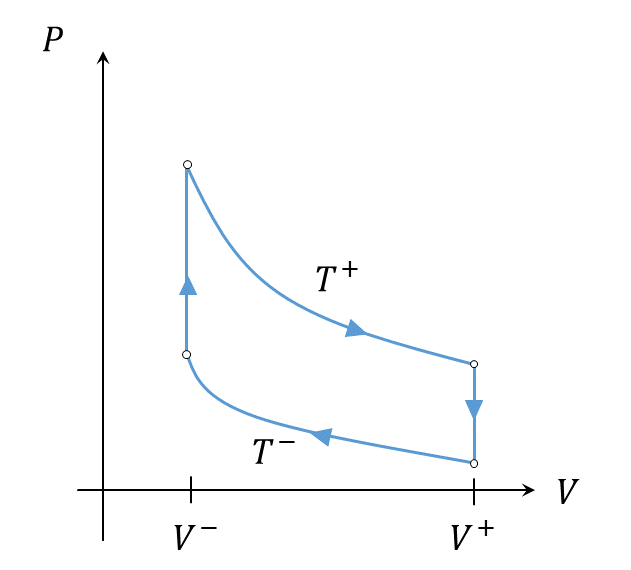
\includegraphics[scale=0.4]{Diapositiv6.PNG}
\caption{Représentation d'un cycle ditherme dans un diagramme $(P,V)$}
\end{figure}

Le bilan total de cette machine va permettre soit de créer du travail (on aura un cycle moteur) ou de la chaleur (on aura alors une machine frigorifique).\\

On peut alors introduire la \textbf{Relation de Clausius} permettant de faire le lien entre les chaleurs mises en jeux ainsi que l'entropie échangée.\\

\begin{theorem}[Relation de Clausius]
La relation de Clausius mes en lien l'entropie échangée avec la somme des rapports des chaleurs des sources sur leurs températures respectives, tel que
\begin{equation}
S_e = \frac{Q_c}{T_c} + \frac{Q_f}{T_f} \leq 0 %NEMETAN REGARDE ICI C'EST IMPORTANT
\end{equation}
\end{theorem}

Où $Q_f$ et $T_f$ sont la chaleur et la température de la source froide, et pour la source chaude quant à $Q_c$ et $T_c$.\\

Dans le cadre d'un \textbf{cycle de Carnot}, un cycle réversible, on a $\delta S_e=0$ car $\delta S_c=0$. A noter que le cycle de Carnot est le cycle possédant le meilleur rendement et la meilleure efficacité dans le cadre des machines dithermes.\\

\begin{definition}[Efficacité]
On définit l'efficacité d'une machine thermique comme le rapport de l'énergie utile sur l'énergie dépensée
\begin{equation}
e=\frac{\textrm{énergie utile}}{\textrm {énergie dépensée}}
\end{equation}
\end{definition}

Si on généralise, on a
\begin{equation}
\sum \limits _i^{N_i} \frac{Q_i}{T_i} \leq 0
\end{equation}

On notera que l'on peut déterminer la valeur du travail d'un cycle à partir de l'aire dans le diagramme de Clapeyron de notre cycle. Dimensionnellement, on a 
$$[P]\times [V]=N.m^{-2}.m^3=N.m=J=[W]$$
Si on fait un diagramme $(S,T)$, l'aire balayée par notre cycle correspondra à la chaleur. Dimensionnelement, cela coincidera à nouveau puisqu'on a d'une part l'entropie en $J.K^{-1}$ et une température en $K$.

\subsection{Moteurs thermiques}

Les moteurs thermiques sont des machines que l'on utilise quotidiennement, par exemple dans nos voitures.

\begin{definition}[Moteur thermique]

Les moteurs thermiques sont des machines qui possèdent un cycle moteur qui, pour fonctionner nécessite de la chaleur. Ainsi, on a 
$$W < 0\textrm{ ; } Q_c > 0 \textrm{ et } Q_f<0$$

\end{definition}

Schématiquement, on a 
\begin{figure}[H]
\centering
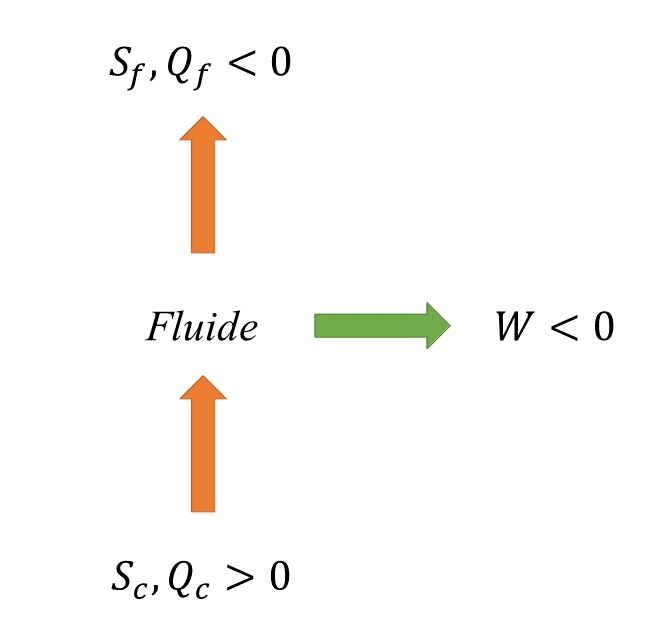
\includegraphics[scale=0.5]{moteur.png}
\caption{Schéma du fonctionnement d'un moteur ditherme ($S_c =$ source chaude et $S_f=$ source froide)}
\end{figure}

\begin{proposition}[Rendement d'un moteur]
On pourra exprimer notre rendement tel que 
\begin{equation}
e_{MT}=-\frac{W}{Q_c} <1
\end{equation}
\end{proposition}

On sait que 
$$\Delta U = W + Q_c+Q_f = 0 \Rightarrow W = -Q_c-Q_f$$

On en déduit que

$$e_{MT}=1+\frac{Q_f}{Q_c}$$

A partir de l'inégalité de Clausius, on peut écrire
$$e= 1 + \frac{Q_f}{Q_c} \leq 1-\frac{T_f}{T_c} <1$$

\begin{proposition}[Cas des transformations réversibles]
Dans les cas de transformations réversibles, on a
\begin{equation}
e=1-\frac{T_f}{T_c}
\end{equation}
\end{proposition}

\subsection{Machines frigorifiques}

Tout aussi courante que les machines thermiques, les machines frigorifiques sont présentes dans nos réfrigérateurs pas exmples, mais aussi dans les systèmes de pompes à chaleur.\\

\begin{definition}[Machine frigorifique]

Une machine frigorifique est une machine à laquelle on va fournir un travail qui va être converti en chaleur. On a alors un fluide caloporteur qui va reçevoir du travail et qui sera en contact avec une source chaude et une source froide auxquels ils cèdera ou récupèrera de la chaleur.
\end{definition}

 Schématiquement, on a 

\begin{figure}[H]
\centering
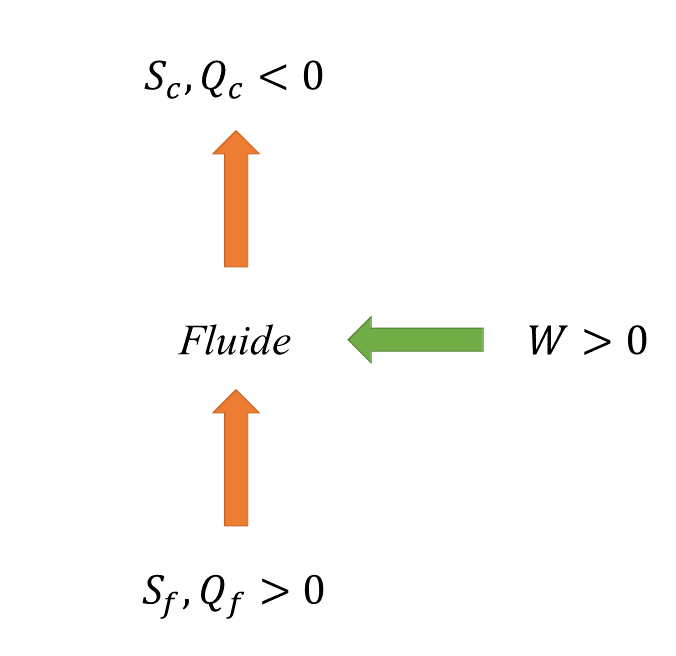
\includegraphics[scale=0.5]{frigo.png}
\caption{Schéma du fonctionnement d'une machine frigorifique ($S_c =$ source chaude et $S_f=$ source froide)}
\end{figure}

\begin{proposition}[Efficacité d'une machine frigorifique]
On pourra exprimer l'efficacité de notre machine frigorifique telle que
\begin{equation}
e_{refre}=\frac{Q_f}{W}\textrm{  ;  } e_{PAC}=-\frac{Q_c}{W}\leq\frac{T_c}{T_c-T_f}
\end{equation}
\end{proposition}

{\color{white}Thermodynamics blank}\\

\begin{remark}

A noter que l'efficacité sera toujours supérieure à 1, en effet, le fonctionnement d'une machine frigorifique part du principe d'extraire de l'énergie à partie d'une source pour la transférer à une autre source en utilisant un travail. 

\end{remark}
